\chapter{Introduction}
\section{Centromere is a specialised locus for chromosome segregation}

 The growth and reproduction of all living organisms rely on cell division. Delivering an intact genome to the daughter cell challenges every dividing cell. Eukaryotes package their genomes into chromosomes, which must be replicated and segregated faithfully during each cell division. Severe diseases, such as cancer, genetic disorder and miscarriage, could arise if chromosome segregation is compromised \citep{Jallepalli2001ChromosomeMystery, Draviam2004ChromosomeStability, Wasielak-Politowska2022ChromosomeAging, Losada2014CohesinBeyond}. 
 
 Centromere is the specialised locus for chromosome segregation, where the chromosome is attached to and pulled by the spindle \citep{Westhorpe2015AMaintenance, McKinley2015TheFunction, Talbert2020WhatCentromere, Fukagawa2014}. First described by \cite{Flemming1882ZellsubstanzZelltheilung} as primary constriction, it is visualised as the intersection point of the iconic X-shaped mitotic chromosome under a microscope. Lack of centromere, or being acentric, leads to chromosome loss during cell division. Although the appreciation of centromere function has been established since its discovery, the molecular feature underneath remained elusive due to the species-to-species variations and the complexity of players involved. \cite{Darlington1936TheEnquiry} therefore recommended defining the centromere in terms of the function rather than the form. Nevertheless, advances in molecular biology shed light on the form of centromere. In most species, the centromeric DNA sequence plays an important but not definitive role in centromere specification \citep{Hoffmann2020, Harrington1997FormationMicrochromosomes, Catania2015SequenceChromatin, Iwata-Otsubo2017, Kasinathan2018Non-B-FormCentromeres, Shukla2018CentromereCycle, Logsdon2019, Murillo-Pineda2020}. It is instead determined epigenetically by the histone H3 variant CENP-A \citep{Warburton1997ImmunolocalizationCentromeres, Vafa1997ChromatinPlate, Earnshaw1985ThreeChromosome, Liu2006MappingCells, Regnier2005CENP-ABubR1, Heun2006, Mendiburo2011, Barnhart2011, Logsdon2015}. The macromolecular protein complex consisting of around 100 subunits, kinetochore, is formed on the centromere to mediate the physical connection between the chromosome and spindle microtubules and act as a signalling hub to monitor the interaction \citep{Musacchio2017AFunction, McAinsh2022TheKinetochores, Cheeseman2014TheKinetochore, Hara2018KinetochoreExit}. Apart from the progress in the form, the mechanisms centromere executing the function have also been elucidated over the years \citep{Tanaka2013, Zhou2020EmergentChromosomes}. In the following sections, the form and function of the centromere will be described in more detail. 

\section{The form of centromere}
\subsection{The genetics}

The structure of centromeric DNA and its functional importance varies dramatically between species. Based on the chromosomal distribution, centromeres are classified as monocentromere, where the centromere is localised at a restricted region of the chromosome, and holocentromere, where the centromere spreads the entire length of the chromosome. Depending on size, the monocentromere can be further divided into point centromere, which contains a short DNA sequence of just over 100 bp, and regional centromere, which could be up to megabases long. The importance of underlying DNA sequences to centromere function could also be very different, ranging from pure genetic to mainly epigenetic. 

Point centromere, with a notable example budding yeast \textit{Saccharomyces cerevisiae}, is the simplest form and the first investigated at the molecular level. A budding yeast centromere consists of three elements \citep{Carbon1984StructuralCEN3}: CDEI, an 8-bp sequence that binds Cfb1 for H3 nucleosome eviction \citep{Niedenthal1993Cpf1I, Henikoff2011EpigenomeResolution}; CDEII, an AT-rich, around 80-bp sequence accommodating a single centromeric nucleosome containing Cse4, the budding yeast CENP-A, for kinetochore assembly \citep{Furuyama2007CentromereYeast, Henikoff2014TheVivo, Krassovsky2012TripartiteYeast} and CDEIII, a 25-bp sequence bound by the CBF3 complex \citep{Yan2018ArchitectureKinetochore}, which recruits the Cse4 chaperon Scm3, the budding yeast HJURP, for Cse4-containing nucleosome deposition \citep{Stoler2007Scm3Localization, Camahort2007Scm3Kinetochore}. Centromere specification is strictly genetic in this organism \citep{Clarke1980IsolationChromosomes, J1986SingleCerevisiae, Kingsbury1991Centromere-dependentVitro}, which could be explained by its unique centromere biology that factors for Cse4 nucleosome deposition are recruited by specific DNA sequences. This is in line with the observation that the exact sequences of CDEI and CDEIII are conserved across all 16 centromeres of budding yeast \citep{Clarke1998Centromeres:Eukaryotes, Baker2005GeneticCerevisiae}. As for the centromeric nucleosome accommodating sequence CDEII, only the length and AT abundance are conserved, supporting the notion from regional centromeres that CENP-A nucleosome binding does not require specific DNA sequences \citep{Bensasson2011EvidenceCentromeres}. The phylogeny indicated that point centromere species evolved from regional centromere species and this transition coincided with the emergence of 2-micron plasmid, a multicopy circular DNA capable of self-propagating in budding yeast \citep{Malik2009MajorComplexity}. Intriguingly, the 2-micron plasmid also uses a single locus called \textit{STB} to assemble a partitioning complex, which includes components of segregation machinery for normal chromosomes such as Cse4 and cohesin, for its association with the spindle microtubule \citep{Rizvi2018TheCerevisiae, Huang2011Evolution, Ghosh2007FaithfulSisters}. The outstanding resemblance led to the hypothesis that the point centromere is the domestication of the self-propagating locus of parasitic plasmids \citep{Malik2009MajorComplexity}. 

The regional centromere is the most common type of centromere. A typical regional centromere is AT-rich and possesses a modular structure composed of a CENP-A-nucleosome-accommodating central core flanked by heterochromatic domains called peri-centromere. The central core usually contains satellite DNA, short sequences repeated a large number of times, whereas the peri-centromere has less patterned sequences \citep{Talbert2020WhatCentromere, McKinley2015TheFunction, Wong2020LessonsChromosomes, Muller2019TheArchitecture}. As one of the fastest-evolving loci across the genome, the precise sequence of the centromere is extremely diverse among species \citep{Melters2013ComparativeEvolution}. Notably, due to the incompatibility of second-generation sequencing and repetitive sequence, deciphering the centromeric DNA sequence has been challenging. In fission yeast \textit{Schizosaccharomyces pombe}, the central core consists of non-repetitive \textit{cc} and inverted repeats \textit{imr} while the peri-centromere possess less ordered \textit{otr} composed of \textit{dg} and \textit{dh} repeats \citep{Chikashige1989CompositeSites, Clarke1993StructureCentromeres, Murakami1991StructureRegion, Nakaseko1986ChromosomeYeast, Nakaseko1987AChromosomes., Steiner1993CentromeresLoci}. Fruit fly \textit{Drosophila melanogaster} has a central core made up of a retroelement-enriched island flanked with AATAT and AAGAG satellites, and peri-centromeric chromatin containing mixed different types of short satellites that are neither conserved among chromosomes nor specific to the centromere \citep{Talbert2018SimpleSpecies, Wong2020LessonsChromosomes, Chang2019IslandsCentromeres}. House mouse \textit{Mus musculus} centromeres are close to telomeres, which is termed acrocentric. The central core and the peri-centromere consist of 120-bp minor satellites and 234-bp major satellites, respectively \citep{Komissarov2011TandemlyGenome, Kuznetsova2006High-resolutionDNA}. Primate including human \textit{Homo sapiens} central core contains 171-bp monomers, named $\alpha$-satellite, arranged into HOR arrays of different lengths, whereas the flanking peri-centromere is built with less structured monomeric $\alpha$-satellites that are less recognisable \citep{Maio1971DNAAethiops, Rosenberg1978HighlySIMIANSIMIANSIMIANSIMIANSIMIAN, Manuelidis1978ComplexDNAs, Manuelidis1978ChromosomalDNAs, Aldrup-MacDonald2014TheGenomics, Logsdon2021The8}. Unlike the point centromere, the centromeric DNA sequence is neither sufficient nor necessary for the function of the regional centromere \citep{McKinley2015TheFunction}. The former was indicated by the observations that the dicentric chromosomes due to the fusion of two normal chromosomes only assembled centromeric proteins, such as CENP-A, at one of the two endogenous centromeres \citep{Earnshaw1985ThreeChromosome, Steiner1994AYeast, Higgins2005EngineeredPlasticity, Sato2012EpigeneticChromosomes, Sullivan1995IdentificationCentromeres, Lange2009IsodicentricPalindromes}. The latter was evidenced by the fact the ectopic centromere, neocentromere, can form on chromosomal regions whose sequences bear little similarity with the canonical centromeres \citep{Marshall2008Neocentromeres:Evolution, Voullaire1993ACentromere, Tyler-Smith1999TransmissionGenerations, Amor2004HumanProgress}. The epigenetic notion was later confirmed by the elucidation of the requirement of CENP-A for centromere function and localisation \citep{Warburton1997ImmunolocalizationCentromeres, Vafa1997ChromatinPlate, Liu2006MappingCells, Regnier2005CENP-ABubR1, Heun2006, Mendiburo2011, Barnhart2011, Logsdon2015, Logsdon2019}. However, experimental results that cloned regional centromeric sequences were sufficient to support the inheritance of exogenous DNA suggest a contribution of sequence to \textit{de novo} centromere formation \citep{Hahnenberger1989ConstructionPombe., Haaf1992IntegrationSegregation, Harrington1997FormationMicrochromosomes, Ikeno1998ConstructionChromosomes}. This could partially be explained by the presence of the sequence-specific DNA-binding centromeric protein CENP-B \citep{Masumoto1989ASatellite., Muro1992CentromereBox., Earnshaw1985IdentificationScleroderma}. CENP-B is not essential for the centromere function as evidenced by that CENP-B knockout mice are still viable \citep{Kapoor1998TheMice, Perez-Castro1998CentromericAbnormalities, Hudson1998CentromereWeights}. But the centromere of the Y chromosome, which lacks CENP-B binding sequences called CENP-B box, failed to generate HACs \textit{in vivo} \citep{Harrington1997FormationMicrochromosomes, Grimes2002-SatelliteFormation}, consistent with the idea that centromeric DNA sequences facilitate the establishment of a functional centromere. The molecular mechanism was later uncovered that CENP-B interacts with both CENP-A and the CCAN component CENP-C to facilitate CENP-A deposition and kinetochore assembly \citep{Chardon2022CENP-B-mediatedCentromeres, Fachinetti2013, Fachinetti2015, Fujita2015StableNucleosome}. As mentioned above, the repetitiveness of centromeric sequences is a conserved feature in various regional centromere species and therefore evolutionarily preferred. Moreover, newly positioned centromeres from speciation, the ENCs, tend to gradually acquire repetitive sequences over time \citep{Rocchi2011CentromereMammals, Kasai2003ChromosomeEvolution}. The hypothesised mode of action is that younger sequences were inserted at the central core, pushing the old sequences towards the flank \citep{Locke2011ComparativeGenomes, Piras2010UncouplingEquus, Ventura2001CentromereEvolution, Kalitsis2012TheCentromere}, which was supported by the recently revealed complete human centromere sequences \citep{Logsdon2021The8}. The evolutionary preference for repetitive sequences also implied its importance to centromere function. It is speculated that tandem repeats might prevent the CENP-A domains from sliding along the centromere over cell cycles \citep{Nergadze2018BirthDomains}. 

Holocentromere refers to the situation where a diffused centromere extends along the whole length of the chromosome instead of a localised one \citep{Guerra2010NeocentricsRules}. It is often seen in flowering plants, insects, arachnids, and nematodes, including the model organism roundworm \textit{Caenorhabditis elegans} \citep{Wong2020LessonsChromosomes}. In mitosis, the holocentromere resides at the poleward faces of the chromosome whereas there is less of a common feature for meiosis \citep{Maddox2004HoloerElegans, Buchwitz1999AElegans, Marques2016HolocentromereHolocentromeres}. At the DNA sequence level, satellites and retrotransposons are enriched in the genome of holocentromere species but they lack an outstanding pattern as in regional centromere species \citep{Kang2016DifferentialElimination, Heckmann2013TheOrganization, Marques2016RestructuringPubera}. In beak-sedge \textit{Rhynchospora pubera} and \textit{C. elegans}, CENP-A nucleosomes do indicate a preferred association with certain DNA sequences \citep{Marques2016HolocentromereHolocentromeres, Gassmann2012AnElegans, Steiner2014HolocentromeresHotspots}. But the fact that these sequences are also actively transcribed suggests the possibility that CENP-A nucleosomes are preferentially loaded at these sites due to their accessibility created by the transcription factors. Indeed, when assessing the importance of DNA sequences for centromere formation in \textit{C. elegans}, it was found that the inheritance of WACs and generation of functional holocentromeres were independent of the DNA sequences used \citep{Stinchcomb1985ExtrachromosomalElegans, Yuen2011RapidEmbryos}. Interestingly, holocentromere has emerged multiple times independently in evolution, termed as convergent evolution in Genetics \citep{Guerra2019MonocentricFamily, Drinnenberg2014RecurrentInsects, Melters2012HolocentricAnalysis}, suggesting a selective force favouring the phenotype. It is unclear what the driver is but one hypothesis is that holocentromere can prevent the loss of fragmented chromosomes due to ionising radiation \citep{Zedek2018HolocentricLand}. Besides the three types of centromere mentioned above, there exists another variety where a few large distinct centromeric domains co-exist on a chromosome, called meta-polycentromere, which is recognised as the intermediate of holocentromere evolution \citep{Neumann2012StretchingDomains}. 

\begin{figure}[htbp]
  \centering
  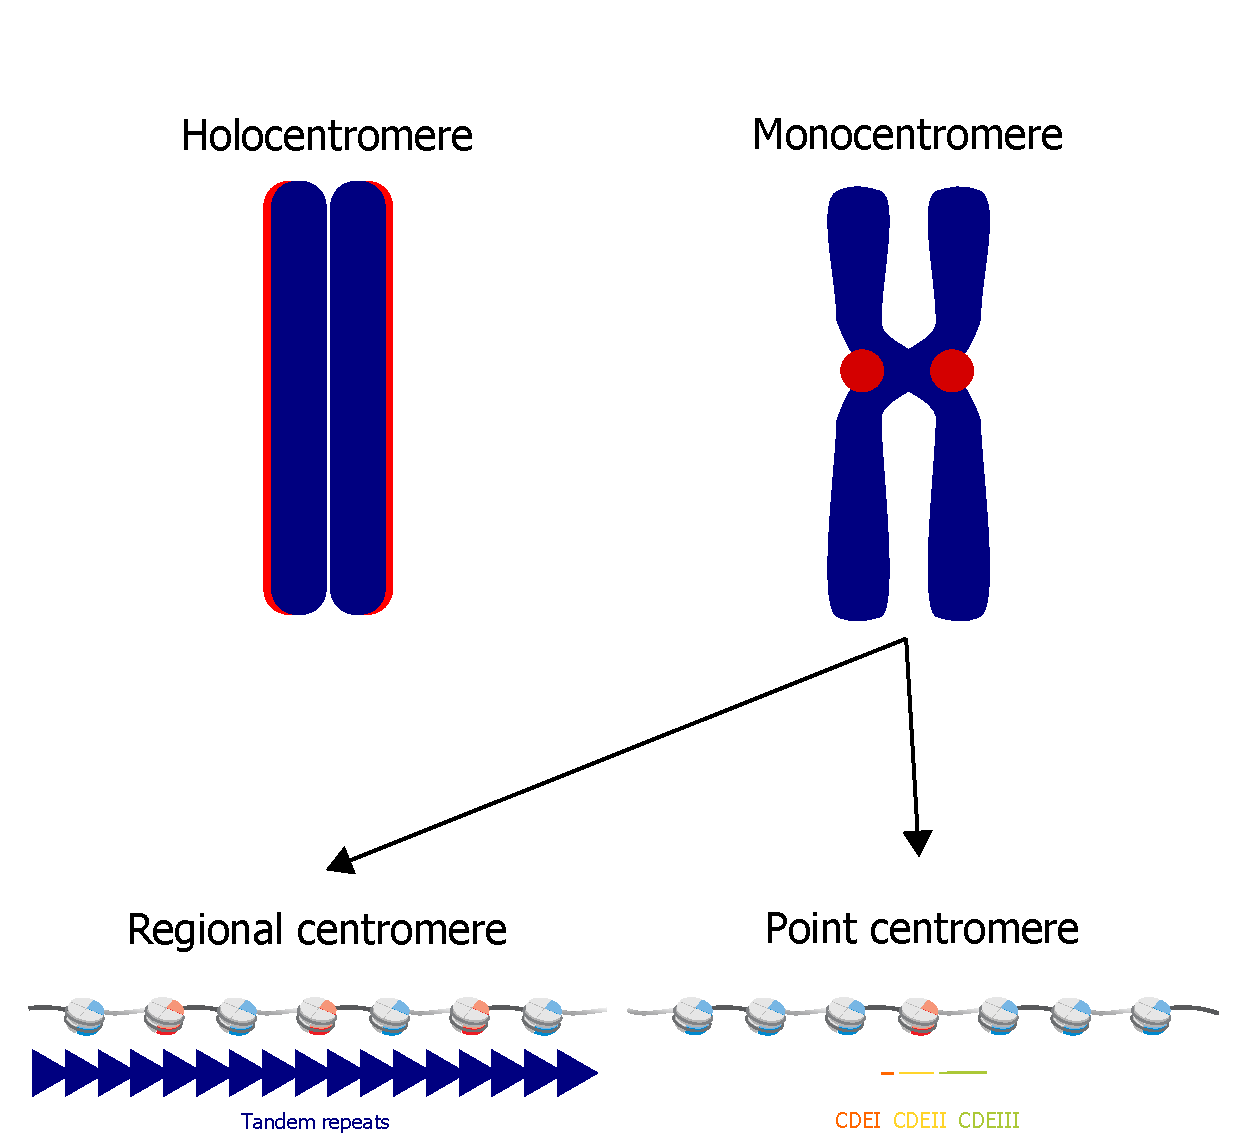
\includegraphics[width=0.9\textwidth]{chapter1/figures/centromere types.pdf}
  \caption[Different types of centroemres]{Different types of centroemres. Broadly, centromeres can be classified into holocentromere or monocentromere, depending on whether a diffused or localised centromere (red) is assembled on the chromosome (blue) under a microscope. Based on the length of DNA sequences and the number of CENP-A nucleosomes, monocentromere can be further divided into regional centromere or point centromere. A regional centromere usually possesses repetitive DNA sequences up to megabases in length and a large number of CENP-A nucleosomes. A point centromere is only composed of over 100 bp DNA sequences and one single CENP-A nucleosome. }
  \label{fig:cenTypes}
\end{figure}

Another common feature of centromeric DNA is the presence of non-B form DNA \citep{Kasinathan2018Non-B-FormCentromeres}, which refers to DNA structures other than the canonical one, such as hairpins and i-motifs. The former has been observed in humans, \textit{Drosophila melanogaster}, old-world monkeys and budding yeast while the latter has been seen in \textit{Drosophila dodeca} and humans \citep{Koch2000NeocentromeresDNA, Ferrer1995CentromericStructures, Catasti1994UnusualCentromeres}. <10-bp dyad symmetries found in many organisms are thought to be responsible for the formation of non-B form DNA. Notably, it is not the case for great apes and mice \citep{Kasinathan2018Non-B-FormCentromeres}. Nevertheless, non-B form DNA can still be detected by permanganate-seq in both species \citep{Kouzine2017Permanganate/S1Genome, Kouzine2013GlobalLymphocytes}. This was attributed to an alternative mechanism where their unique CENP-B boxes are bound by CENP-B, which is thought to induce DNA bending and the formation of non-B form DNA. In line with the idea, the human Y chromosome, which lacks CENP-B boxes, does possess short dyad symmetries \citep{Kasinathan2018Non-B-FormCentromeres}. The extent of effect and mechanism by which non-B form DNA contributes to centromere formation are not known. But it is speculated to facilitate HJURP localisation because the Holliday junction that HJURP binds \textit{in vitro} \citep{Kato2007ActivationCells} might represent short cruciforms enriched at centromeres \textit{in vivo} \citep{Kasinathan2018Non-B-FormCentromeres}. 

\nomenclature{CDE}{Centomere DNA Element}
\nomenclature{CBF}{Centromeric DNA Binding Factor}
\nomenclature{ENC}{Evolutionarily New Centromere}
\nomenclature{HOR}{Higher-Order Repeat}
\nomenclature{HAC}{Human Artificial Chromosome}
\nomenclature{WAC}{Worm Artificial Chromosome}
\nomenclature{i-motif}{intercalated motif}

\subsection{The epigenetics}

As mentioned above, early work with dicentric chromosomes and neocentromeres implied an epigenetic nature of the centromere. In most organisms, the DNA sequences are neither sufficient nor necessary for centromere function. The defining feature of a centromere is instead attributed to the presence of CENP-A-containing nucleosomes. Discovered as the antigen recognised by the 'anti-centromere' antibodies from patients of the autoimmune disease CREST syndrome, CENP-A is found to be enriched at the centromere \citep{Earnshaw1985IdentificationScleroderma}. Subsequent work identified CENP-A to be a variant of histone protein H3 \citep{Palmer1987AHistones, Palmer1990TheNuclei, Palmer1991PurificationHistone., Palmer1985KinetochoreMononucleosomes, Sullivan1994HumanCentromere., Buchwitz1999AElegans, Henikoff2014TheVivo, Takahashi2000RequirementYeast}. Extensive evidence pointed to the determining role of CENP-A in centromere specification. Apart from the canonical centromeres, it is always present at both the active centromeres of dicentric chromosomes \citep{Earnshaw1985ThreeChromosome} and neocentromeres \citep{Marshall2008Neocentromeres:Evolution}. The assembly of the kinetochore, the centromere effector, is strictly dependent on CENP-A \citep{Fachinetti2013, Liu2006MappingCells, Regnier2005CENP-ABubR1}. Moreover, artificial tethering of CENP-A to ectopic loci is sufficient to generate functional centromeres that mediate kinetochore-microtubule interactions and direct chromosome segregation \citep{Heun2006, Mendiburo2011, Barnhart2011, Logsdon2015, Logsdon2019, Roure2019}. 

The distinct biochemical characteristics of CENP-A form H3 have been suggested to account for its ability to confer centromere specification and kinetochore assembly. At the sequence level, CENP-A possesses an N-terminal tail not only largely different from H3 \citep{Sullivan1994HumanCentromere.} but also poorly conserved among species \citep{Goutte-Gattat2013PhosphorylationFunction} and a histone-fold domain that bears 62\% identity with H3. The first loop and second $\alpha$-helix of the histone-fold domain are collectively called CATD for their necessity in the centromeric localisation of CENP-A \citep{Black2007}. Consistently, the chimeric protein of H3 introduced with CATD is capable of being enriched at the centromere \citep{Black2007a}. The dependence of centromere targeting on CATD has been attributed to its interaction with the CENP-A chaperone HJURP \citep{Zhou2011StructuralScm3, Bassett2012, Hu2011StructureHJURP, Shuaib2010HJURPCentromeres}, which is responsible for the deposition of new CENP-A. This region has also been found to directly bind the CCAN component CENP-N \citep{Logsdon2015, Carroll2010, Carroll2009} and, together with the extreme C-terminus, mediate the interaction with the kinetochore assembly 'blueprint' CENP-C \citep{Carroll2010, Kato2013Spt6H3, Guse2011, Walstein2021}. At the structural level, CENP-A nucleosomes are more compact compared to H3 nucleosomes due to the physical properties of CATD \citep{Black2004, Sekulic2010}. The importance of this unique structure to centromere formation is implicated by the result that mutating residues within CATD that are responsible for the structural difference from H3 nucleosomes severely compromised the centromeric localisation of CENP-A \citep{Sekulic2010}. Furthermore, chromatin with CENP-A nucleosomes has a more condensed structure, likely via CENP-C and CENP-N \citep{Panchenko2011, Geiss2014, Zhou2022}. 

As with other epigenetics marks, CENP-A nucleosomes are challenged by cell cycle events and have to be properly propagated at the same locus over the generations. More importantly, errors in centromere propagation will be directly translated into inaccurate chromosome segregation, which leads to genome instability \citep{McClintock1939TheMeiosis, Koshland1987ACerevisiae}. The molecular mechanisms by which CENP-A is propagated are still under active research. The current knowledge of this topic will be introduced in Chapter 2 in detail. In brief, CENP-A nucleosomes are diluted in S phase because of DNA replication and replenished in anaphase or the next G1 of each cell cycle. The replenishment of new CENP-A nucleosomes depends on a positive feedback loop, consisting of CENP-C, HJURP, the MIS18 complex and deposited CENP-A, and a permissive chromatin environment. Mechanisms exist to ensure the resistance of CENP-A nucleosomes to chromatin remodelling events other than DNA replication, resulting in an extremely low turnover rate. The specificity of CENP-A to the centromere is mediated by 'sculpting' mechanisms, which selectly destabilise CENP-A nucleosomes outside centromeric chromatin. 

\nomenclature{CREST}{Calcinosis, Raynaud phenomenon, Esophageal dysmotility, Sclerodactyly and Telangiectasia}
\nomenclature{CATD}{CENP-A-Targeting Domain}

\subsection{The kinetochore}

Proteins carry out nearly all cellular functions. The same applies to the centromere, where the macromolecular protein assembly formed \textit{in situ} called kinetochore, which was originally an equivalent term to centromere \citep{Sharp1921IntroductionCytology, Darlington1936TheEnquiry} but later assigned to the protein complex, is responsible to execute its functions \citep{McAinsh2022TheKinetochores, McKinley2015TheFunction, Musacchio2017AFunction}. Moreover, the formation of a kinetochore in turn reshapes the spatial conformation of centromeric and peri-centromeric chromatin \citep{McAinsh2022TheKinetochores}. Thus, understanding the assemblage of the kinetochore is the key to building up the connection between the form and function of the centromere.

To achieve the highly-demanding, complicated functions of the centromere (to be introduced in Chapter 1 Section 1.3), the kinetochore has evolved an astonishing complexity. For example, in humans, multiple copies of about 100 different proteins are arranged into several self-organising subassemblies to constitute the kinetochore \citep{Cheeseman2014TheKinetochore}. \cite{McAinsh2022TheKinetochores} classified the kinetochore into four subassemblies (Figure~\ref{fig:KTSchematics}), ordered by their proximity to the underlying DNA, namely subassembly I, the CENP-A nucleosomes themselves and the DNA-binding CENP-B; subassembly II, the protein complex called CCAN that recognises CENP-A nucleosomes and stays at the centromere independent of the cell cycle stage, which can also be addressed as ICEN or the inner kinetochore; subassembly III, the critical interface that mediates the interaction with the microtubules called KMN-S network, which can also be termed as the outer kinetochore and subassembly IV, a fibrous corona-shaped structure facilitating the proper microtubule binding, which is consisted of RZZ-S complexes, motor proteins and SAC components. On top of this, another layer of complexity exists that the composition and stoichiometry of the kinetochore show abundant dynamics in response to the kinetochore-microtubule attachment status and the cell cycle stages. For instance, subassembly IV is only assembled on kinetochores unattached to microtubules and the presence window of subassembly III is from prophase to anaphase in animal cells \citep{Hara2020DynamicsProgression}. The components and regulations of each subassembly will be discussed in the following paragraphs with the exception of subassembly I, as they have been introduced in the previous sections. 

\begin{figure}[htbp]
  \centering
  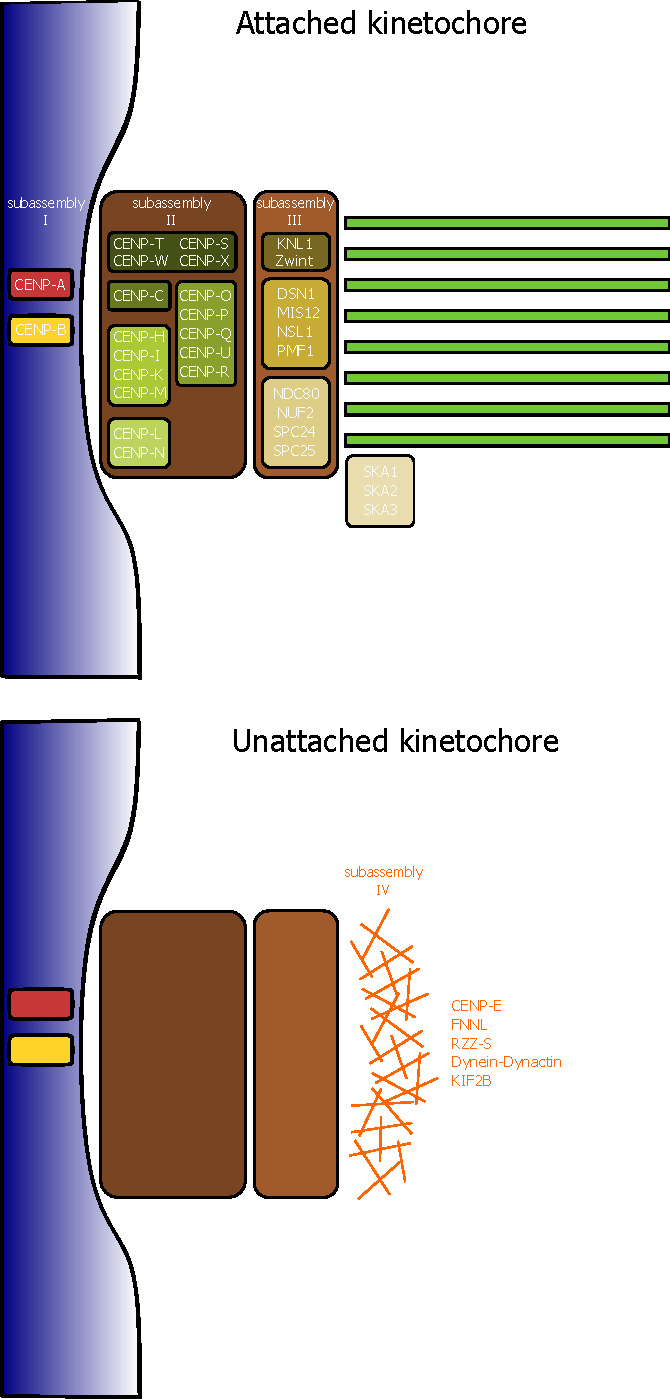
\includegraphics[width=0.9\textwidth]{chapter1/figures/kinetochore.pdf}
  \caption[Schematics of human kinetochore]{Schematics of human kinetochore. The human kinetochore is divided into four subassemblies as described by \cite{McAinsh2022TheKinetochores}. Moving away from centromeric chromatin, subassembly I contains CENP-A and CENP-B. Subassembly II, the inner kinetochore, consists of five subcomplexes, namely CENP-C, CENP-LN, CENP-HIKM, CENP-TWSX and CENP-OPQUR. Subassembly III, the outer kinetochore, is composed of KNL1, MIS12, NDC80 and SKA complexes. On unattached kinetochores, subassembly IV, the corona, forms, which comprises CENP-E, FNNL complex, RZZ-S complex, DD and KIF2B. }
  \label{fig:KTSchematics}
\end{figure}

In human cells, subassembly II, or the CCAN, is composed of 16 different proteins and can be further divided into five subcomplexes \citep{Foltz2006, Izuta2006ComprehensiveCells, Okada2006}. Central to its assembly is CENP-C \citep{Milks2009DissectionAssembly, Przewloka2011CENP-CAssembly}. Although classified in subassembly II, CENP-C is recognised as the 'blueprint' \citep{Walstein2021, Klare2015CENP-CKinetochores} of the whole kinetochore because it sequentially, from N- to C-terminus, contains a MIS12 complex (assembly III) binding site \citep{Screpanti2011DirectKinetochore, Gascoigne2011, Petrovic2016StructureKinetochores}, CCAN subcomplexes (assembly II) binding sites \citep{Klare2015CENP-CKinetochores, McKinley2015, Pentakota2017DecodingCENP-N, Nagpal2015} and CENP-A nucleosomes (assembly I) binding sites \citep{Carroll2010, Kato2013ACENP-C}. With the scope of CCAN, CENP-C interacts with CENP-HIKM and CENP-LN \citep{Klare2015CENP-CKinetochores, McKinley2015, Pentakota2017DecodingCENP-N, Nagpal2015}. Recent cryo-EM data on human CCAN bound to a CENP-A nucleosome revealed that, alongside the CENP-A nucleosome, the CCAN excluding CENP-C forms a gate-like structure wrapping the linker DNA, with CENP-C connecting the two structures. Within the gate-like structure, CENP-OPQUR and CENP-HIKM formed two pillars; CENP-LN formed the arc and CENP-TWSX formed the base \citep{Yatskevich2022StructureNucleosome, Pesenti2022StructureOrganization}. Despite the low level of sequence conservation, budding yeast CCAN, Ctf19 complex, indicated a highly similar structure to human CCAN by cryo-EM \citep{Yatskevich2022StructureNucleosome, Pesenti2022StructureOrganization, Hinshaw2019TheYeast, Yan2019StructureNucleosome}, suggesting a potential generality of eukaryotic kinetochore assembly principles and that the large kinetochores of higher eukaryotes might simply be multiple copies of budding yeast kinetochores \citep{Walstein2021, McAinsh2022TheKinetochores}. However, the importance of the CCAN is compromised by the non-essentiality of the components. In budding yeast, only 3 out of 14 components are required for cell viability \citep{DeWulf2003HierarchicalSubcomplexes, Fernius2009EstablishmentCsm3, Measday2002Ctf3pKinetochore, Ortiz1999AKinetochore, Pot2003Ch14pKinetochore}. In human cells, variable results existed due to the acuteness and completeness of protein depletion and the types of cells used \citep{Foltz2006, McKinley2015, Nguyen2021DifferentialPathways, Pesenti2018ReconstitutionNDC80, Raaijmakers2018BUB1Compromised}. The non-essentiality of the CCAN components and varied requirements of each component for different species might be due to the complexity of the network allowed a large degree of freedom and led to flexibility throughout evolution. 

Sometimes referred to as the KMN-S network, subassembly III is built from four subcomplexes, KNL1, MIS12, NDC80 and SKA complexes \citep{DeWulf2003HierarchicalSubcomplexes, Theis2009ComparativeDivision, Bharadwaj2004IdentificationComplex, McCleland2003TheActivity, Desai2003KNL-1Elegans, Obuse2004AZwint-1, Wigge2001TheSegregation, Westermann2003ArchitectureCore, Cheeseman2004ATension, Cheeseman2006TheKinetochore, Nekrasov2003InteractionsCerevisiae, Pinsky2003AnKinase, Kline2006, Welburn2009TheMotility, Gaitanos2009StableSka3/C13Orf3}. It is localised on subassembly II the inner kinetochore, facing the opposite direction of DNA, hence is also called the outer kinetochore, and directly mediates the interaction between the kinetochore and microtubules. The KNL1 complex is the signalling hub of the cell cycle checkpoint monitoring the status and correctness of kinetochore-microtubule attachment, which is termed SAC (to be introduced in Chapter 1.3.1). It is a heterodimer composed of KNL1 and ZWINT, with the structure and function of the former well studied whereas that of the latter largely remained unknown. From N- to C-terminus, the KNL1 protein possesses a PP1 binding motif that might be under the phospho-regulation by Aurora B \citep{Liu2010RegulatedKinase, Rosenberg2011KNL1/Spc105Checkpoint, Roy2019}, MELT motifs whose phosphorylation by MPS1 forms docking sites for the key SAC signalling proteins BUB1-BUB3 complex \citep{Cheeseman2004ATension, Primorac2013Bub3Signaling, Shepperd2012, Yamagishi2012MPS1/Mph1Components, Vleugel2013ArrayedSegregation, London2012}, which then recruits MAD1-MAD2 complex and BUB3-BUBR1-PP2A complex \citep{Suijkerbuijk2012IntegrationAttachments, Kruse2013DirectProgression, Krenn2012StructuralInteraction}, a ZWINT-binding motif predicted to form a coiled-coil structure \citep{Petrovic2010TheAssembly} and RWD domains interacting with the stalk of MIS12 and NSL1 \citep{Petrovic2014ModularOrganization}. The delicate interplay among kinases and phosphatases present on KNL1 is central to SAC signalling \citep{Saurin2018KinaseKinetochore}. The MIS12 complex forms the linkage connecting subassembly II and the other subcomplexes of subassembly III. Four structural paralogs, DSN1, MIS12, NSL1 and PMF1, compose the Y-shaped complex \citep{Petrovic2010TheAssembly, Petrovic2016StructureKinetochores, Dimitrova2016StructureAssembly, Hornung2011MolecularComplex, Maskell2010MolecularComplex}. The tips of the Y interact with the CCAN \citep{Screpanti2011DirectKinetochore} while the stalk binds both the KNL1 and NDC80 complexes \citep{Petrovic2014ModularOrganization}. The interaction between the MIS12 complex and CCAN relies on the direct binding of MIS12 protein to CENP-C, which requires the phosphorylation of DSN1 by Aurora B which exposes the binding site \citep{Kim2015, Akiyoshi2013TheYeast, Bonner2019EnrichmentAssembly, Hara2018MultipleKinetochores, Rago2015DistinctCENP-T, Zhou2017PhosphorylationMitosis}. This requirement has been proposed to prevent kinetochore assembly by non-centromeric CENP-C. The NDC80 complex, together with the SKA complex, is responsible for the capture of spindle microtubules \citep{Cheeseman2006TheKinetochore, Wimbish2020Hec1/Ndc80Interface, DeLuca2006KinetochoreHec1}. It consists of an NDC80-NUF2 and an SPC24-SPC25 heterodimer. The two dimers possess a very similar structure composed of a globular head and a coiled-coil stalk \citep{Wei2006StructureDomain, Wei2005MolecularComponent, Wei2006TheAttachment, Ciferri2005ArchitectureKinetochore, Ciferri2008ImplicationsComplex}, except that NDC80-NUF2 has a break in the stalk, which is believed to provide rotational freedom \citep{Tang2013Ndc80Motif}. The SPC24-SPC25 dimer binds both the MIS12 complex and the CCAN through the interaction between its RWD domains and MIS12 protein or CENP-T. On the opposing end, the CH domain of the NDC80-NUF2 dimer mediates the interaction with microtubules. The NDC80 complex undergoes jackknifing in the absence of microtubule binding \citep{Roscioli2020, Scarborough2019TightMicrotubules}. Evidence has been reported linking this conformational change to the attachment-sensing function of SAC \citep{Wan2009ProteinSite, Aravamudhan2015TheSignalling}. In metazoa, subassembly III of attached kinetochores further contains the SKA complex to enhance microtubule binding \citep{Welburn2009TheMotility, Gaitanos2009StableSka3/C13Orf3, Theis2009ComparativeDivision}. The SKA complex is a W-shaped complex dimerised from trimers comprising SKA1, SKA2 and SKA3, with the microtubule-binding domain of SKA1 located at the tip of the W \citep{Abad2014StructuralComplex, Jeyaprakash2012StructuralInterface, Schmidt2012TheProtofilaments}. The interaction between SKA3 and coiled coils of the NDC80 complex has been shown to facilitate microtubule binding \citep{Abad2016Ska3Domain, Chan2012AuroraInteraction, Helgeson2018HumanAttachments, Zhang2017Ska3Progression}. Although lacking direct orthologs, budding yeast has a functional equivalent to the SKA complex, named the Dam1 complex. It is a heterodecamer that is able to assemble a ring-like structure with other fifteen copies \citep{Jenni2018StructureInterface, Miranda2005TheMicrotubules, Ramey2011TheMicrotubule, Westermann2005FormationComplex}. Two Dam1 complex rings are present on each kinetochore \citep{Kim2017TheRings}. Similar to the SKA complex, the DAM1 complex associates with the kinetochore in the presence of microtubules \citep{Li2002TheKinetochore} and strengthens their interactions \citep{Lampert2013MolecularComplexes, Lampert2010TheComplex, Tien2010CooperationB}. 

First discovered by EM, subassembly IV, or the corona, is a diffuse fibrous structure specific to unattached kinetochores of metazoan cells \citep{Jokelainen1967TheCells}. It is highly dynamic and undergoes expansion or shrinkage depending on the attachment status of the kinetochore \citep{Kops2020CrowningSegregation}. Known proteins showing corona localisation include the RZZ complex, Spindly, DD, CENP-E, CENP-F, MAD1-MAD2 complex and Cyclin B \citep{McAinsh2022TheKinetochores}. The RZZ complex, composed of ROD, ZW10 and ZWILCH, is recognised as the core because its depletion but not the others led to a complete loss of the corona \citep{Rodriguez-Rodriguez2018DistinctExpansion, Kops2005ZW10Kinetochore, Silio2015KNL1-BubsKinetochores, Varma2013SpindleKinetochores, Auckland2020CENP-FCargoes, Currie2018Bub1Cells}. Spindly is recruited to dimerised RZZ complexes via the interaction with ROD \citep{Mosalaganti2017StructureSpindly, Pereira2018Self-AssemblyAttachment, Raisch2022StructureKinetochores}, which requires the farnesylation of Spindly that releases it from autoinhibition \citep{Sacristan2018DynamicMitosis}. The motor proteins DD are subsequently recruited to the complex by Spindly \citep{Mosalaganti2017StructureSpindly}. However, the mechanism by which the RZZ-S complex itself assembles on subassembly III is unknown. Some of the corona-localised proteins have RZZ-S-independent localisation mechanisms \citep{Ciossani2018TheKinases, Rodriguez-Rodriguez2018DistinctExpansion}. The kinesin CENP-E and CENP-F are distantly related paralogs and are recruited via the kinase domain (or the pseudokinase domain for BUBR1) of SAC components BUB1 and BUBR1, which are another pair of paralogs \citep{Ciossani2018TheKinases, Berto2018DisentanglingKinetochores}. Corona-localised MAD1-MAD2 complexes are recruited in a manner independent of the conventional BUB1-dependent pathway \citep{Pereira2018Self-AssemblyAttachment}, suggesting that they represent a distinct pool. Although still elusive, the corona-associated Cyclin B might be responsible for recruiting this pool \citep{Allan2020CyclinCheckpoint}. The expansion of the corona requires the RZZ-S complex whose ROD and ZWILCH are phosphorylated by MPS1 \citep{Rodriguez-Rodriguez2018DistinctExpansion, Sacristan2018DynamicMitosis, Pereira2018Self-AssemblyAttachment}, whereas the shrinkage depends on DD and Spindly \citep{Sacristan2018DynamicMitosis, Gassmann2010RemovalCells, Howell2001CytoplasmicInactivation}. The apparent negative feedback might exist to allow prompt disassembly once proper microtubule attachment is established. The corona is believed to ensure the speedy and accurate establishment of proper kinetochore-microtubule attachment \citep{Kops2020CrowningSegregation}. Through dynamical expansion and shrinkage, it could facilitate lateral capture of unattached kinetochores by astral microtubules, lateral to end-on attachment conversion, microtubule nucleation from the unattached kinetochore and SAC signalling. 

The kinetochore further affects the structural organisation of centromeric and peri-centromeric chromatin. Due to the fact that methods to study the chromatin localisation of proteins and chromosomal conformation rely heavily on sequencing-based technologies, evidence supporting the argument is mainly from the point centromere species budding yeast, whose centromeric and peri-centromeric DNA sequences are non-repetitive. The SMC complex cohesin is found to be enriched at the core centromere and the two peri-centromere borders \citep{Eckert2007TheTension, Fernius2009EstablishmentCsm3, Fernius2013Cohesin-DependentEstablishment, Glynn2004Genome-WideCerevisiae, Weber2004TheBinding}. It is targeted to the centromere by the direct interaction between the cohesin loader Scc2-Scc4 and the CCAN component Ctf19 phosphorylated by DDK \citep{Hinshaw2015StructuralLoading, Hinshaw2017TheComplex}. Later chromosomal conformation study confirmed that an intrachromosomal loop was formed on each side of the core centromere, physically connecting it to the peri-centromeric borders \citep{Paldi2020ConvergentPericentromeres}. This special conformation appeared to be functional as artificial enlarging of the centromeric loops of merely one chromosome was sufficient to increase chromosome segregation errors \citep{Paldi2020ConvergentPericentromeres}. Apart from this, the kinetochore-localised kinase Bub1 recruits the peri-centromeric protein shugoshin Sgo1 and it in turn recruits another SMC complex condensin to the peri-centromeric chromatin, which has been proposed to generate a back-to-back geometry of sister kinetochores that facilitates proper kinetochore-microtubule interactions \citep{Indjeian2007, Verzijlbergen2014}. 

\nomenclature{ICEN}{Interphase CENtromere complex}
\nomenclature{KMN-S}{Knl1, Mis12, Ndc80 and Ska}
\nomenclature{RZZ-S}{Rod-Zw10-Zwilch-Spindly}
\nomenclature{FNNL}{CenpF-Nde1-Ndel1-Lis1}
\nomenclature{EM}{Electron Microscopy}
\nomenclature{MELT}{methionine(M)-glutamic acid(E)-leucine(L)-threonine(T)}
\nomenclature{RWD}{RING finger-containing proteins, WD repeat-containing proteins, and DEAD (DEXD)-like helicases}
\nomenclature{CH}{Calponin Homology}
\nomenclature{DD}{Dynein-Dynactin}
\nomenclature{DDK}{Dbf4-Dependent Kinase}
\nomenclature{SMC}{Structural Maintenance of Chromosomes}

\section{The function of centromere}

The major function, if not the sole one, of the centromere is to segregate chromosomes faithfully. To accomplish this non-trivial task, it adopts a range of delicate strategies. \textbf{a)} chromosomes are attached to the spindle microtubules through the 'search and capture' principle, where microtubules dynamically grow and shrink to find kinetochores and establish attachment once encountered. Kinetochores promote the occurrence of the stochastic event via several mechanisms, such as localising themselves to limited space, changing geometric architecture according to the attachment status (Chapter 1 Section 1.2.3) and nucleating non-spindle microtubules in proximity to facilitate the growth of spindle microtubules. Detailed information on this field can be found in the review by \cite{Renda2021RoleMorphogenesis}. \textbf{b)} During mitosis, the kinetochores of sister chromatids have to be attached to microtubules from the opposite poles of the spindle, which is termed bi-orientation. It has been estimated that bi-orientated kinetochores are under the force of hundreds of \si{\pico\newton} exerted by microtubules \citep{Ye2016ChromosomeKinetochore}. A special architecture is used by the kinetochore to resist such force \citep{Suzuki2014TheStretch}. \textbf{c)} Apart from bi-orientation, which is desired for accurate chromosome segregation, other types of kinetochore-microtubule attachment can be formed during the error-prone process of 'search and capture' \citep{Tanaka2010Kinetochore-microtubuleBi-orientation}. Two mechanisms are known to promote bi-orientation by the centromere. First, as described in Chapter 1 Section 1.2.3, it introduces an intrinsic bias towards bi-orientation by forming a back-to-back geometry of the sister kinetochores. \textbf{d)} Second, if the geometry failed its job, the centromere could identify and resolve the undesired kinetochore-microtubule attachment while halting the cell cycle until the proper one is established \citep{Marston2015}. \textbf{e)} Centromeric cohesion is essential for the bi-orientation of sister chromatids (to be explained in Chapter 1 Section 1.3.2). The centromere has been found to play an important role in establishing cohesion locally, thereby facilitating accurate chromosome segregation \citep{Tanaka2013}. \textbf{f)} In some organisms, with the notable example of budding yeast, the centromere advances its own replication timing, which has been proposed to allow early kinetochore assembly and efficient establishment of attachment to microtubules \citep{Tanaka2013}. \textbf{g)} Another process crucial for the fidelity of chromosome segregation is the compaction of chromatin into mitotic chromosomes, the chromosome condensation \citep{Piskadlo2016NovelCondensation}. At least in budding yeast, the condensation signals have been proposed to be emitted from the centromere and then propagated throughout the chromosome \citep{Leonard2015, Wilkins2014, Kruitwagen2018}, indicating a new dimension where the centromere contributes to proper chromosome segregation. Considering the relevance to the research projects and the fact that some concepts have been mentioned in the texts above, only selected strategies that the centromere adopts to ensure accurate chromosome segregation will be introduced in the following sections. 

\subsection{Correcting erroneous kinetochore-microtubule attachment}

Except for bi-orientation, or amphitelic attachment, other aberrant attachments could occur during the capture of chromosomes by the spindle, including monotelic, syntelic and, in organisms having more than one microtubule per kinetochore, merotelic attachment \citep{Tanaka2010Kinetochore-microtubuleBi-orientation}. To ensure faithful chromosome segregation, centromere exploits an error correction mechanism to resolve such aberrant attachments \citep{Tanaka2022SWAPCorrection}. The outstanding challenge for error correction is to distinguish incorrect attachments from correct ones \citep{Lampson2011SensingFunction}. A unique outcome of bi-orientated sister chromatids is the presence of tension, which is generated by the resistance of cohesion antagonising the bi-directional pulling of microtubules \citep{Nicklas1997HowChromosomes}. Ever since Nicklas' micromanipulation experiments \citep{Nicklas1969CHROMOSOMEChromosomes, Nicklas1963AMovement}, tension has been recognised as the hallmark of bi-orientation used by the cell \citep{McVey2021AuroraSegregation}. The ability of cells to monitor and interpret the status of tension is termed tension sensing \citep{Lampson2011SensingFunction}. 

Tension is found to stabilise kinetochore-microtubule interaction \citep{Nicklas1969CHROMOSOMEChromosomes}. This suggests a trial-and-error mechanism for error correction, where an attachment is unstable and allows the formation of new ones until tension is established \citep{Nicklas1997HowChromosomes, Tanaka2010Kinetochore-microtubuleBi-orientation, Krenn2015TheSignaling}. At the molecular level, various proteins have been indicated to participate in error correction \citep{Tanaka2022SWAPCorrection} but the central role is attributed to the Aurora B kinase \citep{Krenn2015TheSignaling, Lampson2011SensingFunction, McVey2021AuroraSegregation, Hindriksen2017TheLocalization}. Aurora B is a serine/threonine kinase (consensus motif [RK]x[TS][ILV]) \citep{Cheeseman2002Phospho-regulationIpl1p, Francisco1994TypeSegregation} constituting the CPC together with INCENP, Survivin and Borealin \citep{Gassmann2004BorealinSpindle, Romano2003CSC-1ICP-1, Cooke1987TheMitosis.}. CPC has been found to comprise two distinct modules, connected by the scaffold protein INCENP \citep{Carmena2012TheMitosis}. One regulates the localisation of the complex, consisting of the N-terminal CEN-box of INCENP, Survivin and Borealin \citep{Jeyaprakash2011StructuralComplex, Jeyaprakash2007StructureTogether}, and the other one delivers the catalytic activity, containing the C-terminal IN-box of INCENP and the Aurora B kinase \citep{Kang2001FunctionalSegregation, Bishop2002PhosphorylationActivity, Sessa2005MechanismHesperadin}. Aurora B was first discovered in a budding yeast genetic screen for chromosome segregation errors, or the 'increase in ploidy' phenotype (thus the gene is named \textit{IPL1} in the organism) \citep{Chan1993IsolationYeast.}. Subsequent work identified it as a kinase that can phosphorylate kinetochore components to regulate microtubule binding and hence is important error correction \citep{Cheeseman2002Phospho-regulationIpl1p, Francisco1994TypeSegregation, Biggins1999TheYeast, Tanaka2002EvidenceConnections}. Evidence from \textit{Drosophila}, \textit{C. elegans} and vertebrates further confirmed the conclusion \citep{Giet1999Aurora/Ipl1p-relatedKinases}. Later work revealed that multiple kinetochore substrates are phosphorylated by Aurora B in the absence of tension, including NDC80, KNL1, DSN1 and CENP-C \citep{DeLuca2006KinetochoreHec1, Welburn2010AuroraInterface, Zhou2017PhosphorylationMitosis, Bonner2019EnrichmentAssembly}. It is believed that together they enabled a graded response to variable levels of tension \citep{Welburn2010AuroraInterface}. The regulation by Aurora B phosphorylation is best characterised for NDC80. The unstructured, positive charge of the unstructured N-terminal tail of NDC80 is important for microtubule binding \citep{Ciferri2008ImplicationsComplex, Wei2006StructureDomain, Umbreit2012TheDynamics}. Aurora B phosphorylates this region upon a lack of tension, reducing the positive charge. This decreases its affinity for microtubules and caused the release of the attachment \citep{DeLuca2006KinetochoreHec1, DeLuca2011TemporalMitosis, Ciferri2008ImplicationsComplex, Cheeseman2006TheKinetochore}. Aurora B can further modulate attachment by regulating the conformation of microtubule-depolymerizing kinesin MCAK through phosphorylation \citep{Andrews2004AuroraCentromere, Lan2004AuroraActivity}. The centromere regulates the error correction process by controlling the localisation of the CPC \citep{McVey2021AuroraSegregation}. However, apart from this general statement, this area of research is still vague. It is complicated by the detection of CPC at multiple sub-locations around the broad centromeric region \citep{Liang2020Centromere-localizedSegregation, Fuller2008MidzoneGradient, Hadders2020UntanglingMitosis, Broad2020AuroraCells} and the fact that regulating kinetochore-microtubule interaction is only one of the many functions of CPC \citep{Hengeveld2017InnerSilencing, Afonso2019SpatiotemporalCrosstalk, Liang2020Centromere-localizedSegregation, Hadders2020UntanglingMitosis, Broad2020AuroraCells}. It is unclear which pool of CPC is phosphorylating the kinetochore components mentioned above and how it is able to respond to tension. 

Despite the existence of the opposite view \citep{Etemad2015KinetochoremicrotubuleCheckpoint, Tauchman2015StableCells, Kuhn2019MammalianManner, Magidson2016UnattachedCells}, compelling evidence suggested that tensionless attachment also causes a delay in cell cycle progression \citep{Biggins2001TheCheckpoint, Pinsky2005TheKinetochores, Uchida2009KinetochoreCheckpoint, Li1995MitoticCheckpoint, Shonn2000RequirementMeiosis, Stern2001LackYeast, King2007Ipl1p-dependentKinetochores, Maresca2009IntrakinetochoreActivity}. One likely advantage of this is to allow the error correction enough time to function \citep{Marston2015}. The delay has been found to depend on the SAC \citep{Indjeian2005a, Pinsky2005TheKinetochores}, one of the checkpoints monitoring whether certain criteria are met before allowing cells to enter the next stage of the cell cycle. SAC is the metaphase checkpoint that prevents anaphase onset by emitting inhibitory signals from kinetochores with aberrant attachment \citep{London2014, Musacchio2011SpindleDecade, Lara-Gonzalez2021SpindleKinetochores, McAinsh2023PrinciplesSignalling}. The inhibitory signal is generated by a cascade of kinetochore-localised events. It is initiated by localising the key SAC kinase MPS1 to the microtubule-binding outer kinetochore component NDC80 \citep{Pachis2018LeaderMitosis}. \textit{In vitro} studies indicated a preference of MPS1 for NDC80 unattached by microtubules over attached one \citep{Ji2015KinetochoreNdc80C, Hiruma2015CompetitionSignaling}, which is consistent with the task of SAC. Localised MPS1 can phosphorylate the threonine of MELT motifs of the outer kinetochore signalling hub KNL1, which recruits the BUB1-BUB3 complex \citep{London2012, Shepperd2012, Yamagishi2012MPS1/Mph1Components, Primorac2013Bub3Signaling}. This provides the platform for the production of the inhibitory signal mentioned above, which is named the MCC. The MCC is a hetero-tetramer, composed of MAD2, BUBR1, BUB3 and CDC20 \citep{Musacchio2015TheDynamics, Kops2020EvolutionaryEukaryotes}, that aims to sequester the APC/C co-activator CDC20, whose binding to APC/C is required for the E3 ubiquitin ligase APC/C to mark cell cycle proteins for degradation and thus initiate anaphase \citep{Sudakin2001CheckpointMAD2, Hardwick2000MAD3Mad2p, Alfieri2016MolecularCheckpoint, Izawa2015TheAPC/C, Tsang2023AlternativeDuration}. MCC components are recruited separately to different domains of BUB1. From N- to C-terminus, BUB1 interacts with its kinase-catalytically-deficient paralog BUBR1 in the form of the heterodimer with BUB3, which also interacts with CDC20 \citep{Suijkerbuijk2012ThePseudokinase, Tromer2016Phylogenomics-guidedCheckpoint, Overlack2015ACheckpoint, Alfieri2016MolecularCheckpoint}; MAD1-MAD2 hetero-tetramer that a MAD1 dimer is bound by two 'closed' (C)-MAD2, whose interaction with BUB1 depends on the phosphorylation of CD1 domain by MPS1 \citep{London2014Mad1Checkpoint, Ji2017ASignaling, Zhang2017Bub1Signalling, Fischer2021MolecularBub1}; and CDC20 by the ABBA motif \citep{DiFiore2015TheRegulators}. The MCC is then produced on this platform in the following steps. First, an 'open' (O)-MAD2 is recruited to the MAD1-C-MAD2 complex by dimerising with C-MAD2. Second, the O-MAD2 is converted to C-MAD2 via a conformational change with the help of CDC20 \citep{Mapelli2007MADSignaling, Mapelli2007TheCheckpoint, DeAntoni2005TheCheckpoint}. Third, the transition of MAD2 entraps CDC20 and stabilises the interaction with BUBR1-BUB3 \citep{Piano2021CDC20Complex, Lara-Gonzalez2021AKinetochores, Fischer2022JuxtapositionAssembly, Alfieri2016MolecularCheckpoint}. This leads to a 'handover' of CDC20 from BUB1-BUB3 to BUBR1-BUB3, completing the formation of the soluble MCC. It is widely accepted that SAC is activated by unattached kinetochores \citep{London2014, Musacchio2011SpindleDecade, Lara-Gonzalez2021SpindleKinetochores, Musacchio2015TheDynamics}. However, whether a lack of tension is also a direct trigger of SAC is under debate over a long period of time \citep{McVey2021AuroraSegregation, McAinsh2023PrinciplesSignalling}. From a simplism point of view, the absence of, or reduced, tension destabilised the kinetochore-microtubule attachment because of Aurora B kinase activity, naturally generating unattached kinetochores, which activates the SAC. Therefore, the effect should be indirect. However, recent evidence supports a model where Aurora B directly interferes with and enhances SAC signalling. Although the mechanism remains elusive, the localisation of MPS1 to the kinetochore requires Aurora B kinase activity \citep{Ji2015KinetochoreNdc80C, Saurin2011AuroraMitosis, Nijenhuis2013AB}. Aurora B further phosphorylates the RVSF motif of KNL1 to inhibit PP1 binding, whose recruitment is responsible for the de-phosphorylation of MELT motifs and is believed to be key to SAC silencing \citep{Liu2010RegulatedKinase, Roy2019}. Moreover, BUB1 is also reported to be phosphorylated by Aurora B, which is important for MAD1 binding \citep{Roy2022AuroraSignaling}. Thus, it is likely that SAC monitors both unattached kinetochores and a lack of tension. 

\begin{figure}[htbp]
  \centering
  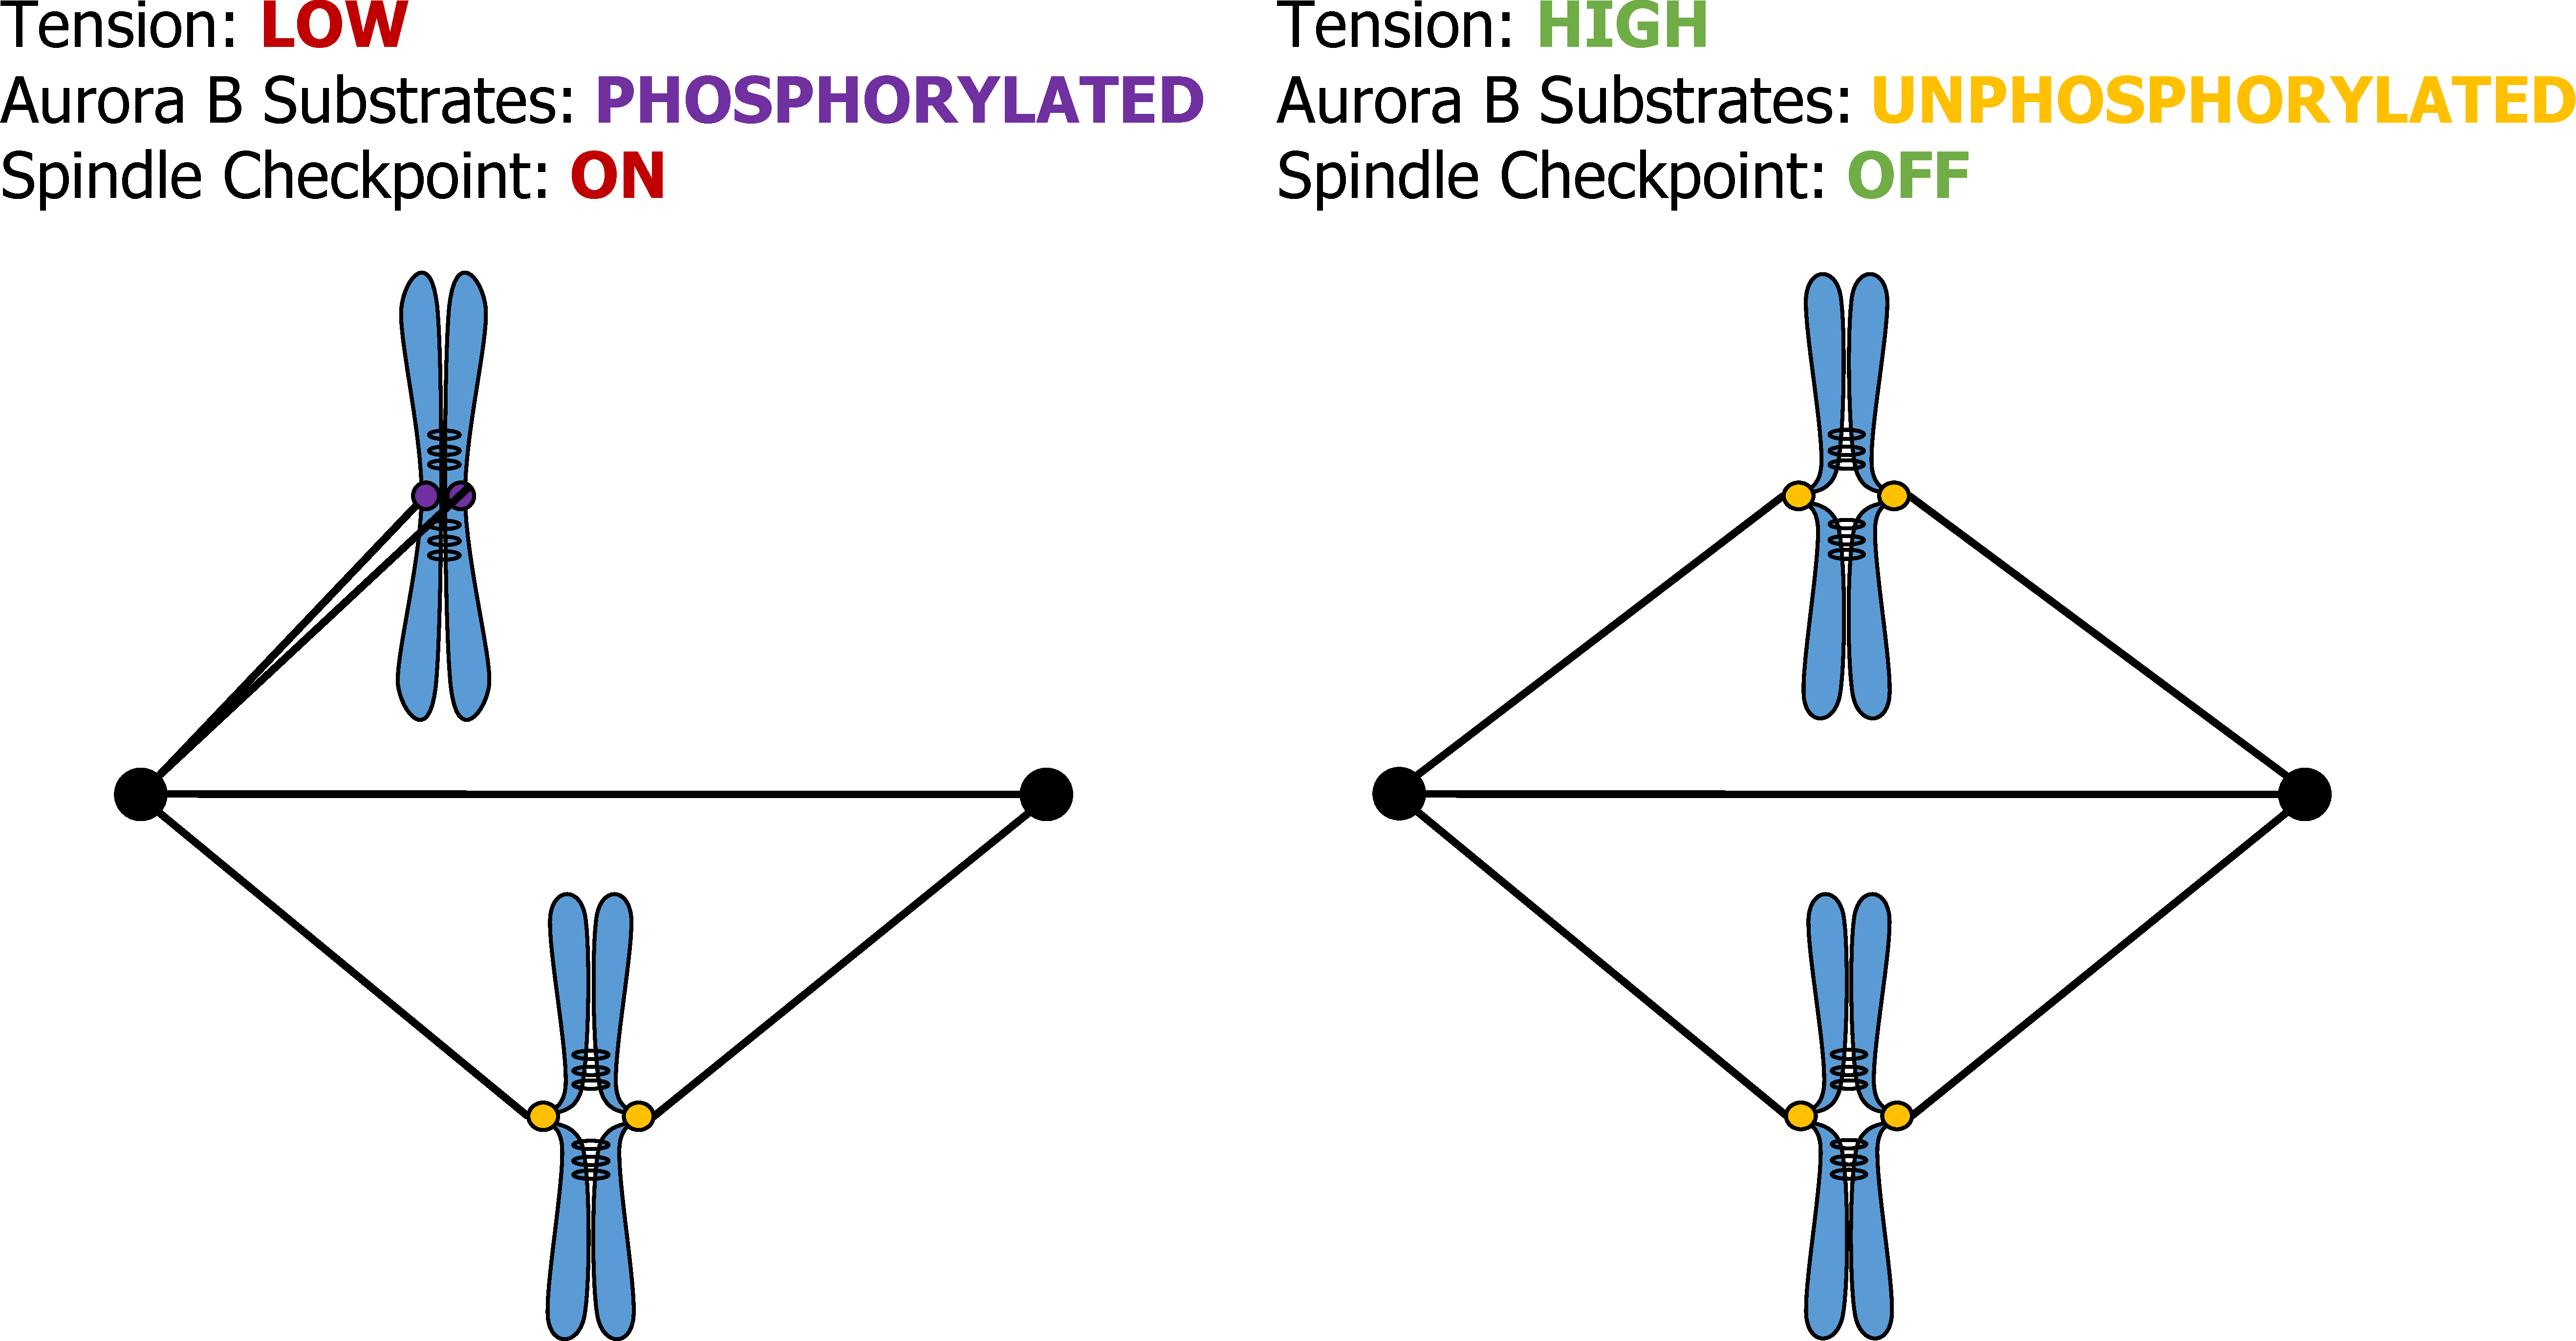
\includegraphics[width=0.9\textwidth]{chapter1/figures/tension sensing schematics.pdf}
  \caption[Tension sensing of the centromere is important for resolving aberrant kinetochore-microtubule attachment]{Tension sensing of the centromere is important for resolving aberrant kinetochore-microtubule attachment. Left: aberrant kinetochore-microtubule attachment is low in tension. The absence of tension triggers the error correction machinery, where the Aurora B kinase phosphorylates kinetochore components to destabilise the erroneous kinetochore-microtubule attachment, enabling new attachment. Error correction can also activate the SAC to prevent anaphase onset by either generating unattached kinetochores or enhancing SAC signalling. Right: Once all pairs of sister chromatids are under tension, The Aurora B substrates are de-phosphorylated. which stabilises the correct kinetochore-microtubule interaction and silences the SAC. }
  \label{fig:tensionSensing}
\end{figure}

\nomenclature{INCENP}{INner CENtromere Protein}
\nomenclature{APC/C}{Anaphase Promoting Complex or Cyclosome}
\nomenclature{ABBA}{cyclin A, BUBR1, BUB1 and Acm1}
\nomenclature{KEN}{lysine(K)-glutamic acid(E)-asparagin(N)}
\nomenclature{CD1}{Conserved Domain 1}

\subsection{Facilitating local cohesion}

Cohesin is the ring-shaped tetramer that is responsible for organising chromosomal architecture. In mitosis, it is composed of two rod-shaped SMC family members SMC1 and SMC3, the kleisin subunit RAD21 and the associated protein SA1/2. The two SMC proteins bind each other, forming the hinge, and the kleisin RAD21 connects them by their head domains, leading to a ring-like structure for cohesin. Despite that the respective mechanism is still under active research, cohesin has been found to organise chromosomes by two distinct modes of action, namely extruding intra-molecular loops and generating sister chromatid cohesion. Centromeric cohesion is essential to the establishment of bi-orientation. As mentioned above, bi-orientation is promoted by geometry-induced bias and error correction, both of which require the existence of centromeric cohesion. Indeed, in both vertebrates and yeasts, cohesin is enriched at the peri-centromeric region and the centromere is important for establishing this local cohesion. 

In vertebrates, the centromere concentrates cohesin locally by preventing its removal from the chromatin. Cohesin loaded onto the chromatin can be removed by a WAPL-dependent pathway, called the prophase pathway. In S phase, cohesin is acetylated in the SMC3 subunit and further bound by PDS5, sororin and WAPL. The association between PDS5 and sororin blocks WAPL from directly interacting with PDS5. However, in prophase, mitotic kinases CDK1 and Aurora B phosphorylate multiple sites of sororin, resulting in its disengagement from PDS5. WAPL is then able to associate with PDS5, together with the phosphorylation of SA2 by PLK, and promote cohesin removal. The peri-centromeric protein SGO1 antagonises this process by two separate mechanisms. First, SGO1 phosphorylated at T346 competes with WAPL for SA2 and RAD21 binding. Second, SGO1 recruits PP2A-B56 to de-phosphorylate sororin, causing its re-association to PDS5 and abolishing WAPL's binding, and SA2. Therefore, cohesin is spared from the prophase pathway at the centromere and forms local enrichment. 

In yeasts, the centromeric enrichment of cohesin is due to promoted local loading. Cohesin loading is mediated by the SCC2-SCC4 complex, which is hence also called the cohesin loader. In budding yeast, DDK-dependent phosphorylation of the inner kinetochore component Ctf19 provides a docking site for the cohesin loader SCC2-SCC4 complex, resulting in the targeted loading of cohesin at the centromere. Notably, there is no detectable prophase pathway in budding yeast. However, the mechanism is not conserved in fission yeast \citep{PeytonJones2022CohesinPombe}. Instead, the peri-centromeric heterochromatin plays an important role. The HP1 ortholog Swi6 recruits DDK, which is required for the local enrichment of cohesin \citep{Bailis2003Hsk1Dfp1Centromeres}. The interaction between Swi6 and SA1/2 ortholog Psc3 is also found to be important for this process \citep{Nonaka2001RecruitmentYeast, Bernard2001RequirementCentromeres, Yamagishi2008}. 

\subsection{Initialising chromosome condensation}

In both mitosis and meiosis, the long thin chromosome strands are re-organised into the iconic thick rod-shaped structures exemplified by cell biology textbooks, which is termed chromosome condensation. It has been proposed to benefit chromosome segregation in various aspects, including spatial compaction, individualisation of sister chromatids and enabling favourable physical properties \citep{Antonin2016ChromosomeMitosis, Piskadlo2016NovelCondensation, Beseda2020MitoticVariability, Takahashi2019FoldingChromosomes}. However, similar to the centromere, despite the cytological and functional appreciation, the form of chromosome condensation (how chromatin is organised in this situation) and how the form achieves the functions still remain elusive. The current model emphasises two distinct pathways for chromosome condensation, with one being the looping of DNA strands mediated by condensin and the other being the intrinsic attraction between nucleosomes regulated by histone PTMs. \cite{Kruitwagen2015} defined the former as compaction and the latter as contraction. Emerging evidence points to a positive role of the centromere in both pathways of chromosome condensation, suggesting a novel way by which the centromere facilitates accurate chromosome segregation. 

Condensin is the pentameric protein complex composed of two SMC subunits, SMC2 and SMC4, and three auxiliary subunits, CAP-D2/3, CAP-G/2 and CAP-H/2. It is highly conserved and structurally similar to the cohesin complex. SMC2 and SMC4 interact at one end called the hinge and their other ends called the heads are linked by the kleisin subunit CAP-H/H2, forming a ring-like structure. This structural similarity brings the possibility that condensin might entrap DNA as cohesin does, which is supported by the evidence from budding yeast. The role of condensin in chromosome condensation is discovered because its depletion resulted in a delay in the process. The mechanism of action is unclear but it is known that condensin is capable of introducing positive supercoils of DNA. It has also been speculated that condensin could multimerise, evidenced by that multiple \textit{Escherichia coli}'s SMC proteins aggregated in proximity under the microscope and that condensin complexes purified from chicken \textit{Gallus gallus} DT40 cells showed populations with different molecular weights. The multimerisation of condensin is suggested to give rise to higher-order structures of chromatin, such as the flower petal structure, further facilitating chromosome condensation. 

The notion that there exist non-condensin-mediated chromosome condensation pathways came from the observation that depletion of condensin did not completely, if at all, abolish chromosome condensation. A series of evidence implicated that inter-nucleosomal interactions might be the alternative to condensin, which is under the regulation of a cascade of histone modifications. It is well characterised by \textit{in vitro} experiments that the acid patch of H2A-H2B could attract the H4 tail from another nucleosome. Subsequent work from budding yeast indicated that this interaction is inhibited by the acetylation of H4-K16. In mitosis, the phosphorylation of H3-T3 by Haspin kinase recruits the CPC to further phosphorylate H3-S10. The latter is then read by the de-acetylase Hst2, which removes H4-K16ac to enable the intrinsic interaction between H4 and neighbouring H2A-H2B. 

Centromere has been indicated to regulate chromosome condensation. Defected chromosome condensation was observed when the holo-centromere of \textit{C. elegan} was disrupted by depleting CENP-A or the loader KNL-2. In line with this, the chromatin level of condensin II was further found to depend on KNL-2. In regional and point centromere species, chromosome condensation is suggested to be initialised at the centromere and then propagated to the chromosome arms. H3-pS10, the contraction indicator, was found to localise at the centromere initially and then spread to the rest of the genome at a similar pace with chromosome condensation in Indian muntjac \textit{Muntiacus muntjak}. Whereas in \textit{D. melanogaster} and budding yeast, it is the compaction that was found to propagate, where condensin was first detected at the centromere and then the distant loci. \cite{Kruitwagen2018} further found in budding yeast that chromosome condensation is regulated by the centromere autonomously in a CPC-dependent manner and that the propagation of it requires signalling cascades involving Sgo1 and Hst2. Thus, the centromere might contribute to chromosome condensation via both compaction and contraction. 

% Interphase chromosomes have to be condensed during mitosis to reduce space occupied, remove sister chromatids catenation, provide physical properties able to withstand forces during movement and therefore facilitate faithful chromosome segregation \citep{Antonin2016ChromosomeMitosis, Piskadlo2016NovelCondensation, Beseda2020MitoticVariability, Takahashi2019FoldingChromosomes}. The current model of chromosome condensation recognises it to be driven by the condensin-mediated compaction pathway and histone-mediated contraction pathway in parallel \citep{Wilkins2014, Kruitwagen2015}. Interestingly, key players from both pathways have been reported to interact with shugoshin or the H2A phosphorylation enabling Sgo1 chromatin association, including Topoisomerase II \citep{Zhang2020FunctioningMitosis} and condensin itself \citep{Verzijlbergen2014, Yahya2020} from the condensin-mediated pathway and CPC \citep{Abad2022MechanisticCPC} from the histone-mediated pathway. This makes Sgo1 and H2A phosphorylation potentially important in chromosome condensation. Indeed, in budding yeast, both compaction and contraction were impaired in the absence of Sgo1 \citep{Kruitwagen2018}. 

\section{Aims of this study}
\subsection{Building a theoretical model for centromere spatial organisation and propagation}
\subsection{Investigating the molecular mechanisms of tension-dependent re-localisation of shugoshin}


However, the key question 'How does tension regulate the phosphorylation of Aurora B substrates?', or the plain language version 'How is tension sense?' has troubled the field. Location-wise, it is unclear whether inter- or intra-kinetochore tension is sensed. At the molecular level, it is not known how a mechanical force is translated into biochemical signals. A number of models that are neither mutually exclusive nor can be easily proven with current experimental techniques have been proposed \citep{McVey2021AuroraSegregation}. 

% coarse grain level intra- vs inter- kt tension
% detailed level many many models not mutually exclusive

% nevertheless, 
% Localization of Aurora B and the CPC is critical for proper chromosome segregation. During prometaphase and metaphase, the CPC localizes at the inner centromere, then relocates to the spindle midzone in anaphase [98] where it plays a role in mitotic exit [99]. Studies in HeLa demonstrated that precise inner centromere localization of the CPC is critical for SAC silencing and preventing premature separation of sister chromatids [100]. However, precise CPC localization was not required for Aurora B correction of erroneous attachments [100]. This separation of function based on localization is supported by recent studies that identified multiple pools of Aurora B. Distinct populations were found localized to the inner centromere, outer centromere proximal to kinetochores, and the outer kinetochore [86,101,102]. Each population was uniquely recruited (see “Kinetochore localization model” section for details) and demonstrates separation functions. The two chromatin-based pools appear to regulate SAC silencing in response to tension, but do not contribute to phosphorylation of erroneous attachments [86,101,102]. These studies suggest that the kinetochore-based population of Aurora B/CPC may be the pool critical for destabilizing incorrect attachments.

% The Two Recruitment Arms That Control Inner Centromere Localization of the CPC
% shugoshin tension-dependent re-localisation might explain tension sensing (act as tension sensor)
% it is not known how shugoshin localisation is regulated by tension

